\documentclass[paper=a4, fontsize=11pt,twoside]{article}

% -------------------------------------------------------------------- 
% General Page Layout
% --------------------------------------------------------------------
\usepackage[a4paper]{geometry} 
\usepackage[parfill]{parskip}
\setlength{\oddsidemargin}{5mm}  % Remove 'twosided' indentation
\setlength{\evensidemargin}{5mm}

% --------------------------------------------------------------------
% Encoding and Language Settings
% --------------------------------------------------------------------
\usepackage[T1]{fontenc} 
\usepackage[utf8]{inputenc}   
% encoding may need to be changed depending on the system
\usepackage[swedish]{babel} 
\usepackage{lipsum} % Lorem Ipsum

% --------------------------------------------------------------------
%  Utilities (colors, links, pictures, ect...)
% --------------------------------------------------------------------
\usepackage{xcolor}
\usepackage{hyperref}
\usepackage{graphicx}
\usepackage{amssymb}
\usepackage{epstopdf}
\usepackage[round]{natbib}
\usepackage{float}
\usepackage{pgfgantt}
\DeclareGraphicsRule{.tif}{png}{.png}{`convert #1 `dirname #1`/`basename #1 .tif`.png}

% -----------------------------------------------------------------------------%
% Title Page / Document Class Definitions (Please Don't Play With This)
% -----------------------------------------------------------------------------%
	
% Table of contents depth = section & subsection
\setcounter{tocdepth}{1}
																								
% Horizontal rule
\newcommand{\HRule}[1]{\rule{\linewidth}{#1}}   															
																											
% Document Number
\newcommand{\documentNumber}[1]{\centering PUSP1742#1 \\[1.0cm]}	 										
																											
% Document Version
\newcommand{\documentVersion}[1]{\centering \small{v.#1} \\[1.0cm]}

% Group Responsible
\newcommand{\documentResponsible}[1]{\centering  Ansvarig Grupp: #1}

% Document Creator Group
\newcommand{\documentCreator}[1]{\centering Uppgjord Av: #1}	 									
																										
% Title
\makeatletter \def\printtitle{ {\centering \@title\par}} \makeatother
																											
% Author .. not really used, but it can stay in case
\makeatletter \def\printauthor{ {\centering \large \@author}} \makeatother
																											
\newcommand{\grouptitlepage}[4]{ 
	\title{
		\documentNumber{#1}																						
		\documentVersion{#2}																				
		\HRule{0.5pt} \\ % Upper rule 
		\LARGE \textbf{\uppercase{#3}} \\
		\large \textbf{\uppercase{ETSF20 Grupp 2}} 
		\HRule{2pt} \\ [1.5cm]    
		\normalsize            
		\documentResponsible{#4} \\ 
		\documentCreator{#4}  
	}																							
	\maketitle																							
	\thispagestyle{empty} 																					
	\newpage 
}
% \grouptitlepage{doc number}{Version Number}{doc title}{group responsible for
% doc}
% --------------------------------------------------------------------------------%
% Title Page / Document Class Definitions (Please Don't Play With This)
% --------------------------------------------------------------------------------%


% \date{}                                            
% Activate to display a given date or keep commented for current date


% -------------------------------------------------------
% DOCUMENT START (YOU CAN IGNORE EVERYTHING ABOVE HERE)
% -------------------------------------------------------
\begin{document}

% -------------------------------------------------------
% Title Page START
% -------------------------------------------------------
\grouptitlepage
% the \# typesets a # character into the document, you will need to replace them
% in yourdocuments. This is a template, just plug in what you need between the
% {}s. Document Code Number (same as time reports)
{09}
% Document Version Number
{0.1}
% Document Title
{Veckoplanering}
% Group Responsible For Document
{(PG) Projekt Grupp}
% -------------------------------------------------------
% Title Page END
% -------------------------------------------------------
%\tableofcontents
% WRITE THINGS BELOW HERE


\section{Gantt schema}
\begin{figure}[H]
\centering
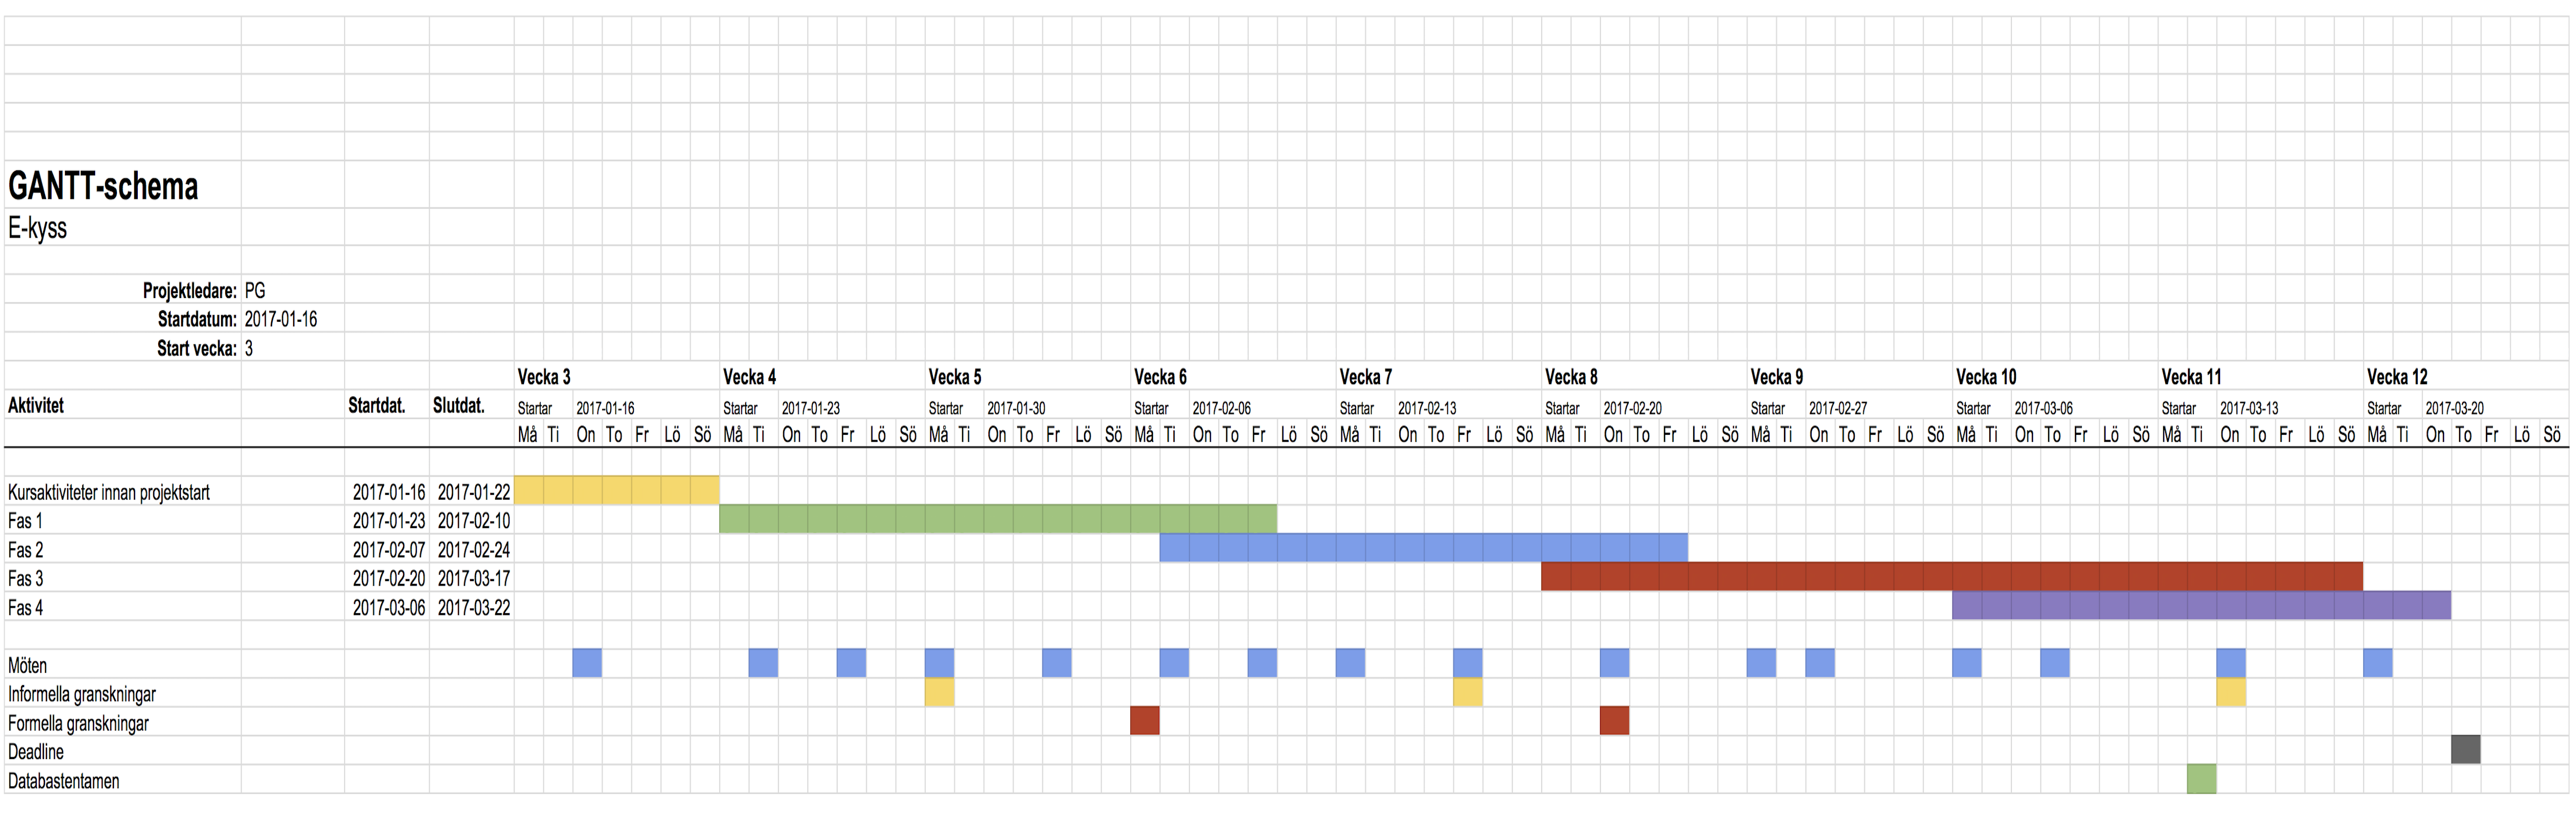
\includegraphics[width = 17cm]{e-kyss-gantt.png} %height=6cm,
\caption{Gantt schema}
\end{figure}


\section*{Vecka 5:}
Denna vecka sker arbete med SDP, SRS och SVVS.\\
\subsection*{Monday 30 Jan 2017}
	12:00 - 13:00: Informell granskning\\
\subsection*{Wednesday 1 Feb 2017}
	8:00 - 13:00: Arbetstid\\
\subsection*{Thursday 2 Feb 2017}
	13:00 - 17:00: Arbetstid när man inte har labb\\
\subsection*{Friday 3 Feb 2017}
	8:30 - 10:00 Arbetstid\\
	15:00 - 16:00 Arbetstid\\



\section*{Vecka 6:}
Denna vecka sker omarbete efter formell granskning och start av STLDD och
SVVI.\\
 \subsection*{Monday 6 Feb 2017}
	15:00 - 16:00: Formell granskning\\
\subsection*{Tuesday 7 Feb 2017}
	10:00 - 12:00 Arbetstid: Åtgärder och smygstart fas 2\\
	12:00 - 13:00 Lunchmöte\\
\subsection*{Wednesday 8 Feb 2017}
	8:00 - 17:00: Arbetstid: Åtgärder och start fas 2\\
\subsection*{Thursday 9 Feb 2017}
	12:00 - 17:00 Arbetstid när man inte har labb\\
\subsection*{Friday 10 Feb 2017}
	12:00 - 13:00 Lunchmöte\\
	13:00 - 18:00 Arbetstid\\




\section*{Vecka 7:}
Denna vecka fortsätter arbetet med STLDD och SVVI. Smygstart fas 3.\\
\subsection*{Monday 13 Feb 2017}
	12:00 - 13:00 Lunchmöte\\
\subsection*{Tuesday 14 Feb 2017}
	10:00 - 15:00 Arbetstid med tid för mässING\\
\subsection*{Wednesday 15 Feb 2017}
	8:00 - 13:00 Arbetstid\\
\subsection*{Thursday 16 Feb 2017}
	10:00 - 17:00 Arbetstid när man inte labbar\\
\subsection*{Friday 17 Feb 2017}
	12:00 - 13:00 Informell granskning\\



\section*{Vecka 8:}
Denna vecka sker omarbete efter informell och senare formell granskning. Start
fas 3.\\
 \subsection*{Monday 20 Feb 2017}
	12:00 - 17:00 Arbetstid\\
\subsection*{Wednesday 22 Feb 2017}
	8:00 - 11:00 Arbetstid\\
	11:00 - 12:00 Formell granskning\\
	12:00 - 13:00 Lunchmöte\\
	13:00 - 17:00 Arbetstid\\
\subsection*{Thursday 23 Feb 2017}
	8:00 - 17:00 Arbetstid\\



\section*{Vecka 9:}
Under denna vecka pågår kodning för fullt. PFR och SSD påbörjas.\\
\subsection*{Monday 27 Feb 2017}
	12:00 - 13:00 Lunchmöte\\
	13:00 - 17:00 Arbetstid\\
\subsection*{Wednesday 1 Mar 2017}
	8:00 - 12:00 Arbetstid\\
	12:00 - 13:00 Lunchmöte\\
	13:00 - 17:00 Arbetstid\\
\subsection*{Thursday 2 Mar 2017}
	12:00 - 17:00 Arbetstid\\
\subsection*{Friday 3 Mar 2017}
	8:00 - 17:00 Arbetstid\\



\section*{Vecka 10:}
Kodning fortsätter, testning påbörjas, SVVR påbörjas.\\
\subsection*{Monday 6 Mar 2017}
	12:00 - 13:00 Lunchmöte\\
	13:00 - 17:00 Arbetstid\\
\subsection*{Tuesday 7 Mar 2017}
	8:00 - 17:00 Arbetstid\\
\subsection*{Wednesday 8 Mar 2017}
	12:00 - 17:00 Arbetstid\\
\subsection*{Thursday 9 Mar 2017}
	8:00 - 12:00 Arbetstid\\
	12:00 - 13:00 Lunchmöte\\
	13:00 - 17:00 Arbetstid\\



\section*{Vecka 11:}
Åtgärder efter informell granskning och test. Debugging.\\
\subsection*{Wednesday 15 Mar 2017}
	9:00 - 10:00 Informell granskning\\
	10:00 - 11:00 Möte\\
	11:00 - 18:00 Arbetstid\\
\subsection*{Thursday 16 Mar 2017}
	8:00 - 17:00 Arbetstid\\
\subsection*{Friday 17 Mar 2017}
	8:00 - 17:00 Arbetstid\\



\section*{Vecka 12:}
Avslutande vecka.\\
\subsection*{Monday 20 Mar 2017}
	8:00 - 10:00 Arbetstid\\
	12:00 - 13:00 Lunchmöte\\
	13:00 - 17:00 Arbetstid\\
\subsection*{Tuesday 21 Mar 2017}
	8:00 - 13:00 Arbetstid\\
\subsection*{Wednesday 22 Mar 2017}
	8:00 - 17:00 Arbetstid\\
\subsection*{Thursday 23 Mar 2017}
	8:00 - 17:00 DEADLINE\\





\end{document}










